\documentclass{article}
\usepackage{graphicx} % Required for inserting images
\usepackage{caption}
\usepackage{subcaption}

\title{Camera Calibration}
\author{Shaunak Kolhe}
\date{April 2023}

\begin{document}

\maketitle

\newpage

\section{Camera Calibration}

Camera extrinsic calibration for the vehicle was done using Kalibr. Each of the three cameras were calibrated using the pinhole model with radial and tangential distortion. Based on the geometry of the rig, the cameras were observed to have a 30\% overlap in frames which made extrinsic calibration easier.
Bag files were recorded with the golfcart in a stationary, and an aprilgrid tag as the calibration target.

\begin{table}[h]
    \centering
    \begin{tabular}{c|c}
        Columns & 6 \\
        Rows & 6 \\
        Tag Size [m] & 0.099 \\
        Tag Spacing & 0.30303
    \end{tabular}
    \caption{April Tag parameters for Calibration Target}
    \label{tab:my_label}
\end{table}

From the intrinsics, the cameras were observed to have a pixel re-projection error between 0.4 to 0.48 pixels. The azimuthal and polar errors from the intrinsics are as shown below.

\begin{figure}
     \centering
     \begin{subfigure}[b]{0.3\textwidth}
         \centering
         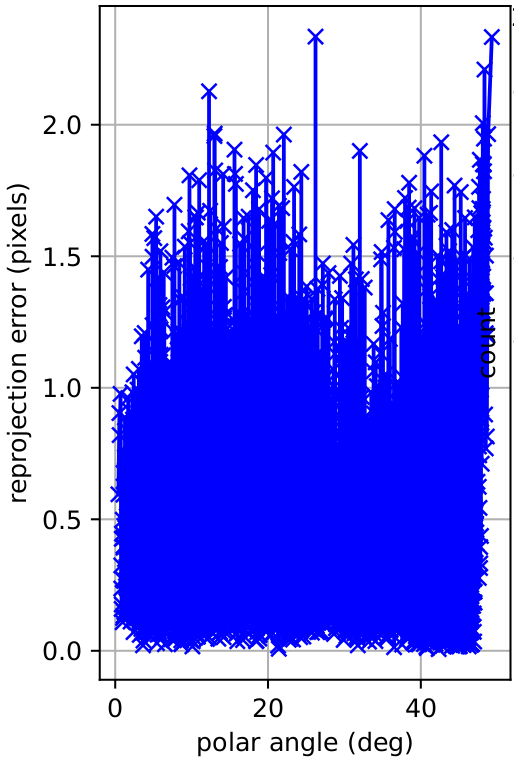
\includegraphics[width=\textwidth]{cam0polar.png}
         \caption{Left\_Cam}
     \end{subfigure}
     \hfill
     \begin{subfigure}[b]{0.3\textwidth}
         \centering
         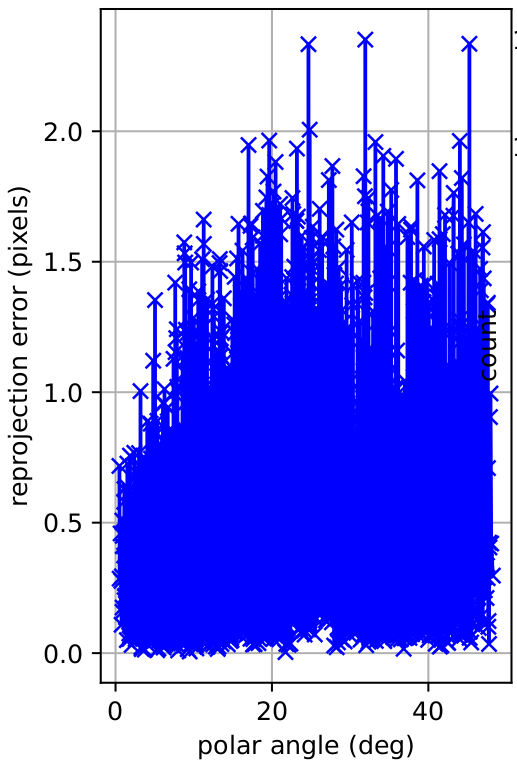
\includegraphics[width=\textwidth]{cam1polar.png}
         \caption{Middle\_Cam}
     \end{subfigure}
     \hfill
     \begin{subfigure}[b]{0.3\textwidth}
         \centering
         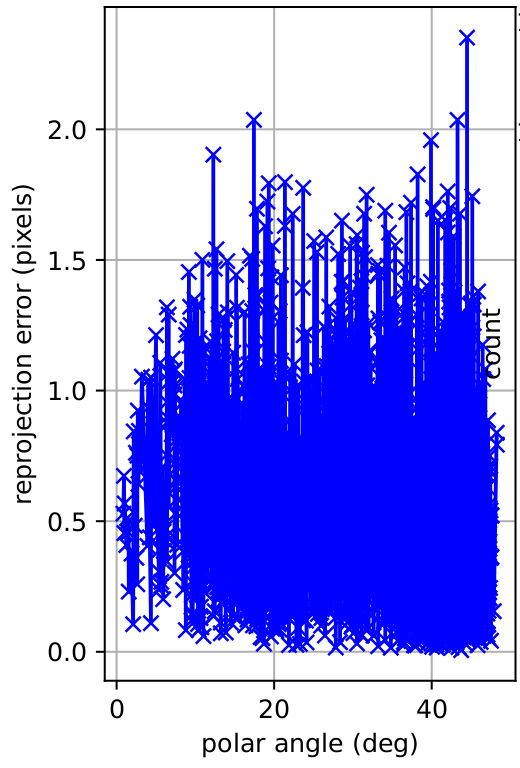
\includegraphics[width=\textwidth]{cam2polar.png}
         \caption{Right\_Cam}
     \end{subfigure}
        \caption{Polar Reprojection error}
    \hfill
     \begin{subfigure}[b]{0.3\textwidth}
         \centering
         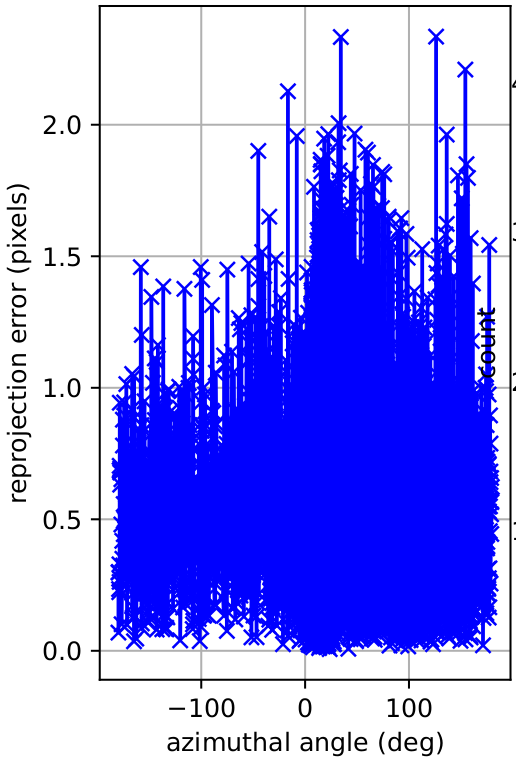
\includegraphics[width=\textwidth]{cam0az.png}
         \caption{Left\_Cam}
     \end{subfigure}
     \hfill
     \begin{subfigure}[b]{0.3\textwidth}
         \centering
         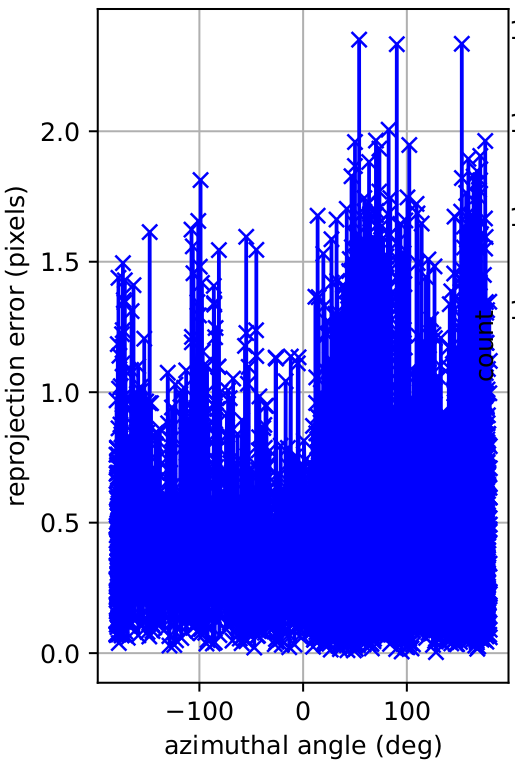
\includegraphics[width=\textwidth]{cam1az.png}
         \caption{Middle\_Cam}
     \end{subfigure}
     \hfill
     \begin{subfigure}[b]{0.3\textwidth}
         \centering
         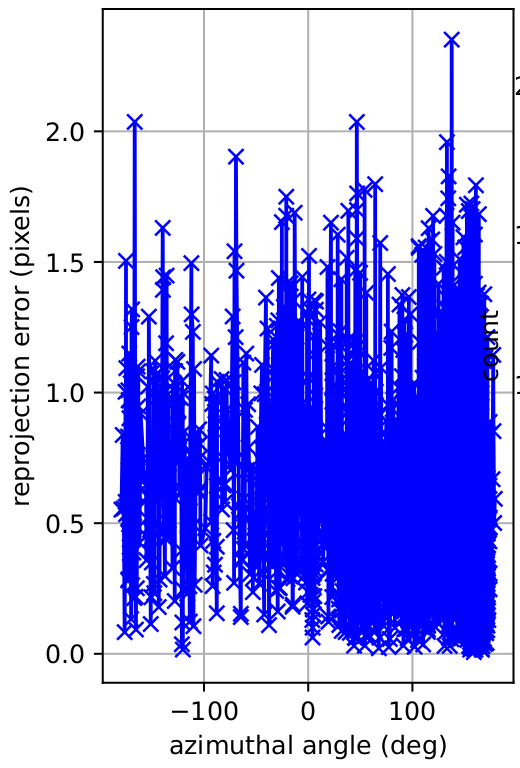
\includegraphics[width=\textwidth]{cam2az.png}
         \caption{Right\_Cam}
     \end{subfigure}
        \caption{Azimuthal Reprojection error}
\end{figure}

\newpage

The extrinsics of the camera system can be shown as

\begin{figure}[h]
    \centering
    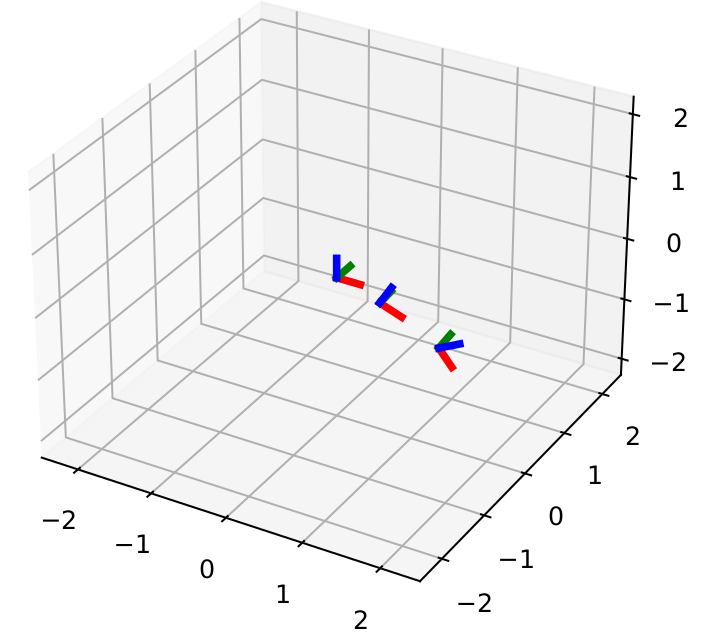
\includegraphics[scale=0.5]{CamSys.png}
    \caption{Camera System}
\end{figure}

The transformations from the cameras are given in a cam chain file as generated by Kalibr, which can be found here [link]

\end{document}
